\documentclass[tikz,border=2pt]{standalone}
\usepackage{amsmath}
\usetikzlibrary{arrows.meta}
\begin{document}
% Population shares A = [[0.9,0.2],[0.1,0.8]], x_0 = (1,0)^T: x_t = (1/3)(2,1)^T + (1/3)(0.7)^t (1,-1)^T.
% The component along (2,1)^T (lambda = 1) stays fixed; the one along (1,-1)^T shrinks by 0.7 each period.
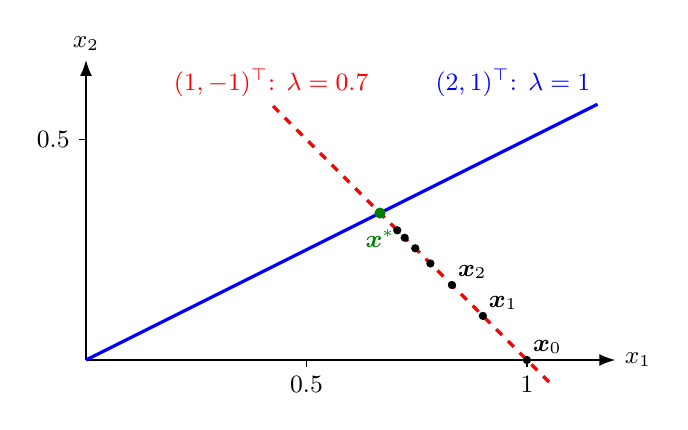
\begin{tikzpicture}[font=\small, >={Latex[length=2mm]}, x=5.6cm, y=5.6cm]
  \draw[->] (0,0) -- (1.2,0) node[right] {$x_1$};
  \draw[->] (0,0) -- (0,0.68) node[above] {$x_2$};
  \foreach \x in {0.5,1} \draw (\x,0) -- (\x,-0.015) node[below] {$\x$};
  \draw (0,0.5) -- (-0.015,0.5) node[left] {$0.5$};
  % eigen-directions
  \draw[blue, very thick] (0,0) -- (1.16,0.58) node[above left, inner sep=2pt] {$(2,1)^{\top}$: $\lambda=1$};
  \draw[red, very thick, dashed] (1.05,-0.05) -- (0.42,0.58) node[above, inner sep=2pt] {$(1,-1)^{\top}$: $\lambda=0.7$};
  % iterates
  \foreach \p in {(1.0000,0.0000), (0.9000,0.1000), (0.8300,0.1700), (0.7810,0.2190), (0.7467,0.2533), (0.7227,0.2773), (0.7059,0.2941)}
    \fill[black] \p circle (1.5pt);
  \node[anchor=south west, inner sep=2pt] at (1.0,0.0) {$\boldsymbol{x}_0$};
  \node[anchor=south west, inner sep=2pt] at (0.9,0.1) {$\boldsymbol{x}_1$};
  \node[anchor=south west, inner sep=2pt] at (0.83,0.17) {$\boldsymbol{x}_2$};
  \fill[green!50!black] (0.6667,0.3333) circle (2pt);
  \node[green!50!black, anchor=north, inner sep=2pt] at (0.6667,0.31) {$\boldsymbol{x}^*$};
\end{tikzpicture}
\end{document}
